% ADD THIS HEADER TO ALL NEW CHAPTER FILES FOR SUBFILES SUPPORT
\documentclass[../CLthesis.tex]{subfiles}
\graphicspath{{\subfix{../images/}}}
\usetikzlibrary{arrows.meta, shapes.geometric, positioning, fit, backgrounds}
% END OF SUBFILES HEADER

\begin{document}
\chapter{Methods}%
\label{chap:methods}

This thesis addresses three research questions about anti-Christian hate speech in East Asian online discourse: who the targets are, how hatred is expressed, and what moral motivations underlie it. Each question requires a different analytical lens, and no single method is sufficient to answer all three. We therefore adopt a modular, sequential pipeline in which each stage builds on the outputs of the previous one.

The pipeline proceeds in four stages. First, topic modelling with \texttt{BERTopic} groups the full multilingual corpus into semantically coherent clusters, establishing the thematic map over which all subsequent analyses are conducted. Second, named entity recognition and domain lexicon matching identify the concrete targets of attack within each topic. Third, dependency parsing and LLM-assisted frame classification characterize the rhetorical form of each attack. Fourth, lexicon-augmented vector projection onto Moral Foundations Theory axes asks why different language communities attack Christianity using different moral vocabularies.

\begin{figure}[h]
\centering
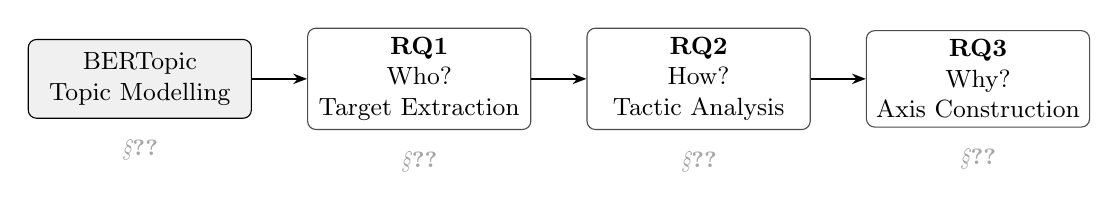
\begin{tikzpicture}[
  node distance=0.5cm and 0.7cm,
  box/.style={rectangle, rounded corners=3pt, draw=black, fill=gray!12,
              text width=2.6cm, align=center, minimum height=1.0cm,
              font=\small},
  rqbox/.style={rectangle, rounded corners=3pt, draw=black!70, fill=white,
                text width=2.6cm, align=center, minimum height=1.0cm,
                font=\small},
  arr/.style={-{Stealth[length=5pt]}, thick},
  lbl/.style={font=\footnotesize\itshape, text=gray!70}
]

\node[box] (bt)  {BERTopic\\Topic Modelling};
\node[rqbox, right=of bt] (r1) {\textbf{RQ1}\\Who?\\Target Extraction};
\node[rqbox, right=of r1] (r2) {\textbf{RQ2}\\How?\\Tactic Analysis};
\node[rqbox, right=of r2] (r3) {\textbf{RQ3}\\Why?\\Axis Construction};

\draw[arr] (bt) -- (r1);
\draw[arr] (r1) -- (r2);
\draw[arr] (r2) -- (r3);

\node[lbl, below=0.15cm of bt] {§\ref{sec:bertopic}};
\node[lbl, below=0.15cm of r1] {§\ref{sec:rq1}};
\node[lbl, below=0.15cm of r2] {§\ref{sec:rq2}};
\node[lbl, below=0.15cm of r3] {§\ref{sec:rq3}};

\end{tikzpicture}
\caption{Overview of the analytical pipeline. BERTopic provides the shared thematic scaffold; each subsequent stage addresses one research question.}
\label{fig:pipeline-overview}
\end{figure}

% ------------------------------------------------------------------
\section{Topic Modelling with BERTopic}
\label{sec:bertopic}
% ------------------------------------------------------------------

Topic modelling is used to discover the thematic structure of the corpus without imposing predefined categories. We use \texttt{BERTopic} \citep{grootendorst_bertopic_2022}, a neural topic modelling framework that combines transformer-based sentence embeddings, dimensionality reduction via UMAP \citep{mcinnes2020umapuniformmanifoldapproximation}, and density-based clustering via HDBSCAN \citep{campello_density-based_2013} to produce coherent, human-interpretable topics. Compared to classical methods such as Latent Dirichlet Allocation \citep{blei2003latent}, BERTopic captures richer semantic structure because it operates on dense contextual embeddings rather than bag-of-words representations, and it naturally handles the noise and short-text characteristics typical of social media data.

To ensure comparability across languages and avoid corpus-size dominance effects, we randomly sample up to 2,000 hate-speech instances from each language subset (Chinese, Japanese, and English). For languages with fewer than 2,000 available instances, all data are retained.

\subsection{Multilingual Sentence Embeddings}

All documents — Chinese, Japanese, and English — are encoded using \texttt{intfloat/multi\allowbreak lingual-e5-large-instruct} \citep{wang2024multilinguale5textembeddings}, a large multilingual encoder pre-trained on a diverse mixture of supervised and weakly supervised multilingual data. The E5-large model maps texts from all three languages into a shared 1024-dimensional embedding space, making cross-lingual semantic comparisons possible without translation.

To further reduce residual language-specific distributional shifts, we apply a post-hoc embedding alignment step in which vectors are mean-centered separately within each language group and then L2-normalized before joint topic modelling. This simple normalization-based alignment strategy follows common practices in cross-lingual embedding calibration and space alignment \citep{artetxe2018robust,conneau2018wordtranslation}.

\subsection{Dimensionality Reduction and Clustering}

To extract meaningful thematic patterns, we employ a two-stage pipeline consisting of non-linear dimensionality reduction followed by density-based clustering:

\begin{itemize}
    \item \textbf{Dimensionality Reduction}: The 1024-dimensional aligned embeddings are projected into a 5-dimensional latent space using \texttt{UMAP}. To prioritize the preservation of local topological structures and facilitate dense cluster formation, we set \texttt{n\_neighbors=30}, \texttt{min\_dist=0.0}, and utilize the \texttt{cosine} metric.
    
    \item \textbf{Density-Based Clustering}: The reduced embeddings are processed via \texttt{HDBSCAN} with a \texttt{min\_cluster\_size} of 20 and \texttt{min\_samples} of 5. We utilize the \textit{excess-of-mass} (\texttt{eom}) method with \texttt{cluster\_selection\_epsilon=0.05} to refine cluster membership.
\end{itemize}

\noindent \textbf{Rationale and Noise Handling}: Compared to partition-based methods like K-Means, \texttt{HDBSCAN} is preferred as it (i) handles clusters of arbitrary shapes and varying densities, (ii) obviates the need for a pre-defined cluster count, and (iii) robustly identifies outliers \citep{campello_density-based_2013}. Consequently, documents assigned to the \texttt{-1} label are treated as stochastic noise and excluded from subsequent analysis to ensure thematic consistency.

\subsection{Keyword Extraction and Topic Labelling}

Within BERTopic, topic-level keywords are extracted using a class-based TF-IDF (c-TF-IDF) procedure \citep{grootendorst_bertopic_2022}, which weighs terms by their importance within a topic relative to the full corpus. To handle the morphological structure of Chinese and Japanese, documents are pre-tokenized before keyword extraction: Chinese text is segmented using \texttt{jieba}, and Japanese text is tokenized using \texttt{Janome}. A multilingual stop-word list is applied during vectorization, combining standard English stop words from NLTK with Chinese and Japanese stop-word files, augmented by a domain-specific list of high-frequency but semantically uninformative religious terms.

After the initial BERTopic run, topic labels are further refined using a GPT-4o-mini representation model \citep{openai2024gpt4technicalreport}. For each topic, the three documents closest to the cluster centroid (as measured by cosine distance) are selected as representative texts and passed to the LLM together with the top keywords, which then generates a concise descriptive label. This hybrid approach — combining c-TF-IDF for keyword extraction with LLM-based labelling for interpretability — produces more semantically coherent topic names than either method alone.

\subsection{Cluster Quality Assessment}

We assess clustering quality along two dimensions. First, the noise ratio (proportion of documents assigned to topic $-1$) should fall within a reasonable range of 10--40\%, reflecting meaningful cluster structure without excessive rigidity. Second, we compute per-topic language entropy to quantify cross-lingual mixing: $H_t = -\sum_{l} p_{tl} \log p_{tl}$, where $p_{tl}$ is the proportion of language $l$ in topic $t$. Topics with high entropy are those in which hate speech from all three language communities converges around a shared semantic theme, and their prevalence serves as the primary validity metric for the multilingual alignment procedure.

\begin{figure}[h]
\centering
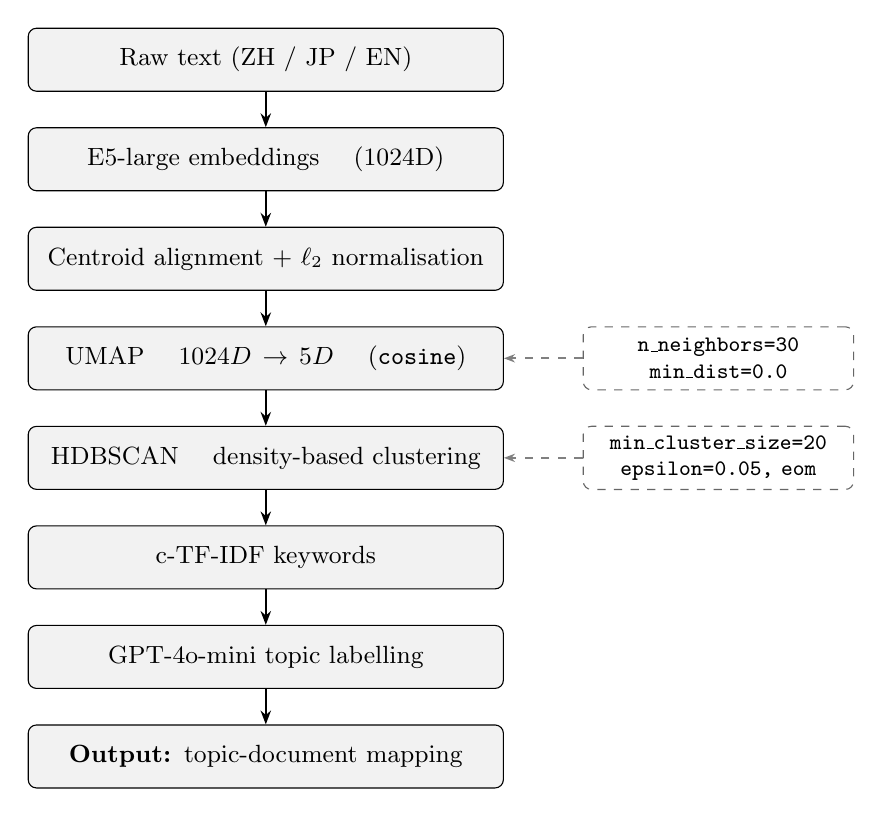
\begin{tikzpicture}[
  node distance=0.45cm,
  box/.style={rectangle, rounded corners=3pt, draw=black, fill=gray!10,
              text width=5.8cm, align=center, minimum height=0.8cm, font=\small},
  sidebox/.style={rectangle, rounded corners=3pt, draw=black!60, fill=white,
                  text width=3.2cm, align=center, minimum height=0.8cm,
                  font=\footnotesize, dashed},
  arr/.style={-{Stealth[length=5pt]}, thick},
  sarr/.style={-{Stealth[length=4pt]}, thick, dashed, gray}
]

\node[box] (raw)  {Raw text (ZH / JP / EN)};
\node[box, below=of raw]  (e5)   {E5-large embeddings \quad (1024D)};
\node[box, below=of e5]   (aln)  {Centroid alignment + $\ell_2$ normalisation};
\node[box, below=of aln]  (umap) {UMAP \quad $1024\text{D} \rightarrow 5\text{D}$ \quad (\texttt{cosine})};
\node[box, below=of umap] (hdb)  {HDBSCAN \quad density-based clustering};
\node[box, below=of hdb]  (kw)   {c-TF-IDF keywords};
\node[box, below=of kw]   (llm)  {GPT-4o-mini topic labelling};
\node[box, below=of llm]  (out)  {\textbf{Output:} topic-document mapping};

% side annotations
\node[sidebox, right=1.0cm of umap] (par1) {\texttt{n\_neighbors=30}\\
                                              \texttt{min\_dist=0.0}};
\node[sidebox, right=1.0cm of hdb]  (par2) {\texttt{min\_cluster\_size=20}\\
                                              \texttt{epsilon=0.05, eom}};

\draw[arr] (raw)  -- (e5);
\draw[arr] (e5)   -- (aln);
\draw[arr] (aln)  -- (umap);
\draw[arr] (umap) -- (hdb);
\draw[arr] (hdb)  -- (kw);
\draw[arr] (kw)   -- (llm);
\draw[arr] (llm)  -- (out);

\draw[sarr] (par1.west) -- (umap.east);
\draw[sarr] (par2.west) -- (hdb.east);

\end{tikzpicture}
\caption{BERTopic pipeline. Raw multilingual text is embedded, aligned across languages, reduced, clustered, and finally labelled to produce a topic-document mapping used by all three RQ analyses.}
\label{fig:bertopic-pipeline}
\end{figure}

% ------------------------------------------------------------------
\section{RQ1: Target Identification}
\label{sec:rq1}
% ------------------------------------------------------------------

RQ1 asks who is being attacked in anti-Christian online discourse. The analysis takes the topic-labelled corpus from Section~\ref{sec:bertopic} as input and applies a three-stage extraction pipeline to identify the specific named entities and groups targeted in each document, then aggregates these targets by topic and language.

\subsection{Stage 1 \& 2: NER and Domain Lexicon Matching}

The first two stages of target extraction operate without LLM calls and produce an initial checkpoint. Stage 1 applies transformer-based Named Entity Recognition (NER) using language-specific spaCy models: \texttt{en\_core\_web\_trf} for English, \texttt{zh\_core\_web\_trf} for Chinese, and \texttt{ja\_core\_news\_trf} for Japanese \citep{honnibal2017spacy}. We retain entities belonging to categories that are meaningful in the context of religious attacks: \textsc{person}, \textsc{org}, \textsc{norp} (nationalities, religious, and political groups), \textsc{gpe} (geo-political entities), and \textsc{fac} (facilities) for English; equivalent categories for Chinese and Japanese.

To capture entities that NER misses — particularly collective religious labels and denominational sub-groups that are common in religious hate speech but rare in general NLP training data — Stage 2 applies a domain-specific gazetteer covering 40+ categories (e.g., \textit{Religious Group}, \textit{Church Institution}, \textit{Clergy Role}, \textit{Individual Figures}). This gazetteer was constructed from a combination of prior work on target identification in hate speech \citep{yoder_how_2022, thomson_identity-based_2021} and manual inspection of the most frequent noun phrases in the corpus. Pronouns and generic nouns are filtered out via a blacklist, as are uninformative domain terms (e.g., ``religion,'' ``faith'') that are near-ubiquitous across the corpus and therefore carry no discriminative information about attack targets.

Surface-form variation — specifically English singular/plural alternation (e.g., \textit{Catho\allowbreak lic}/\textit{Catholics}) — is handled at two levels: case-insensitive matching during gazetteer lookup prevents case-variant duplicates within a single document, and substring-aware deduplication further collapses near-identical mentions at the document level. Across-document frequency counts deliberately preserve the singular/plural distinction, as the two forms carry different pragmatic functions in hate-speech targeting (collective-identity label vs.\ individual or adjectival usage), and conflating them via lemmatization would risk masking this difference. High-priority alias merges (e.g., \textit{Jesus Christ} $\rightarrow$ \textit{Jesus}, Unification Church variants $\rightarrow$ 統一教会) are handled explicitly via a curated alias map rather than a general stemmer, ensuring precision on the entities most central to the analysis. Chinese and Japanese do not inflect for grammatical number, so morphological normalization for those languages reduces to character-level alias mapping, which the alias table already covers.

\subsection{Stage 3: LLM Fallback}

Documents that yield no target from Stages 1 and 2 — a non-trivial proportion in Chinese and Japanese, where zero-subject constructions and topic-drop are grammatically normal — are passed to a Gemini API fallback \citep{geminiteam2025geminifamilyhighlycapable}. Given the raw sentence, the model is prompted to identify the most plausible attack target, if any. Asynchronous batch processing with token-bucket rate limiting and exponential-backoff retry is used to manage API quota constraints, and results are cached to disk after each batch to enable checkpoint-resume on failure.

\subsection{Aggregation and Visualisation}

Extracted targets are aggregated by topic and language to produce a frequency-ranked list of attack targets per language community. Cross-language comparisons are made at the topic level: for each topic, the top-5 targets in each language are compared to identify both universal targets (appearing prominently in all three languages) and language-specific targets.

\begin{figure}[h]
\centering
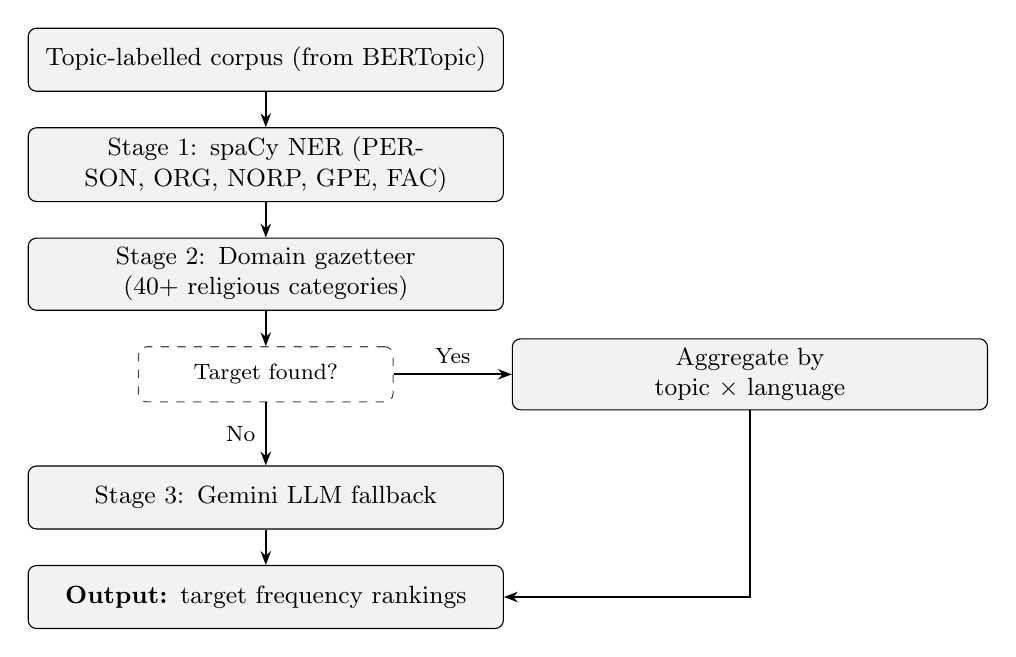
\begin{tikzpicture}[
  node distance=0.45cm and 1.2cm,
  box/.style={rectangle, rounded corners=3pt, draw=black, fill=gray!10,
              text width=5.8cm, align=center, minimum height=0.8cm, font=\small},
  decbox/.style={rectangle, rounded corners=3pt, draw=black!70, fill=white,
                 text width=3.0cm, align=center, minimum height=0.7cm,
                 font=\footnotesize, dashed},
  arr/.style={-{Stealth[length=5pt]}, thick},
  darr/.style={-{Stealth[length=4pt]}, dashed, thick, gray}
]

\node[box] (inp)  {Topic-labelled corpus (from BERTopic)};
\node[box, below=of inp]  (s1)   {Stage 1: spaCy NER (PERSON, ORG, NORP, GPE, FAC)};
\node[box, below=of s1]   (s2)   {Stage 2: Domain gazetteer (40+ religious categories)};

% decision: target found?
\node[decbox, below=of s2]  (dec)  {Target found?};

\node[box, below=0.8cm of dec] (s3)  {Stage 3: Gemini LLM fallback};
\node[box, right=1.5cm of dec] (agg) {Aggregate by\\topic $\times$ language};
\node[box, below=0.45cm of s3] (out) {\textbf{Output:} target frequency rankings};

\draw[arr] (inp) -- (s1);
\draw[arr] (s1)  -- (s2);
\draw[arr] (s2)  -- (dec);
\draw[arr] (dec) -- node[left, font=\footnotesize]{No} (s3);
\draw[arr] (dec) -- node[above, font=\footnotesize]{Yes} (agg);
\draw[arr] (s3)  -- (out);
\draw[arr] (agg.south) |- (out.east);

\end{tikzpicture}
\caption{RQ1 target extraction pipeline. Stages 1 and 2 are rule-based; Stage 3 is an LLM fallback for structurally incomplete sentences (common in Chinese and Japanese).}
\label{fig:rq1-pipeline}
\end{figure}

% ------------------------------------------------------------------
\section{RQ2: Attack Frame Classification}
\label{sec:rq2}
% ------------------------------------------------------------------

RQ2 asks how hatred is expressed — specifically, what rhetorical and thematic frames attackers use to construct anti-Christian discourse. Building on the targets identified in RQ1, the pipeline extracts the predicate--argument structure of hateful statements and classifies each into one of ten attack frame categories.

\subsection{Syntactic Extraction: Three-Layer Strategy}

A key design challenge is that social media text in all three languages frequently lacks canonical subject--verb--object (SVO) structure. Chinese online discourse makes heavy use of zero-subject sentences and topic chains; Japanese routinely drops both subject and object; English social media features imperative sentences and fragmented posts. We therefore adopt a complementary three-layer extraction strategy rather than relying on dependency-parsed SVO triples alone.

Layer 1 applies dependency parsing using spaCy to extract explicit SVO triples from sentences that contain a complete subject and object. This works well for English and a subset of Chinese texts. Layer 2, the predicate window method, handles structurally incomplete sentences: for documents that contain a known attack target but no parseable SVO, we extract all content verbs within a $\pm N$-word window centred on the target entity, filtering out a language-specific stop-verb list. This recovers the predicate--target relationship even when the subject is absent. Layer 3 passes the extracted verb--target pairs from Layers 1 and 2 to a Gemini LLM for frame classification, using a structured prompt with chain-of-thought reasoning that maps each predicate--argument pair to one of the ten frame categories defined below.

\subsection{Attack Frame Taxonomy}
\label{sec:rq2-taxonomy}

The ten-category taxonomy used in this thesis is author-constructed: no prior scheme provided a ready-made classification that covered the full range of anti-Christian discourse across three languages simultaneously. The taxonomy was developed inductively through three rounds of pilot coding on a stratified random sample of 200 documents drawn from the BERTopic corpus (approximately 70 per language). The resulting scheme is also informed by prior theoretical work on hate speech discourse, particularly the explicitness and power dimensions articulated in \citet{matamoros-fernandez_racism_2021}, and by the framing literature's distinction between diagnostic frames (attributing blame) and motivational frames (calling to action) \citep{Mendelsohn_2024}.

The final taxonomy comprises ten categories, defined below with representative examples drawn from the corpus:

\begin{enumerate}
    \item \textbf{Cognitive Manipulation}: Accusations that a religious institution or group uses deceptive psychological techniques — brainwashing, indoctrination, or cult-like mind control — to recruit or retain members, overriding individual rational agency. \textit{Example:} ``Christians assaulted people trying to make use of their new freedom'' (EN); 洗脑 (\textit{brainwash}) directed at 教会 (\textit{church}) (ZH); 狂信的カルト (\textit{fanatical cult}) directed at 統一教会 (\textit{Unification Church}) (JA).

    \item \textbf{Moral Accusation}: Charges that individuals or institutions have violated their own publicly professed moral code --- hypocrisy, abuse of power, or double standards --- framing the target as morally discredited rather than physically dangerous. \textit{Example:} ``They wish to spread their religious beliefs by force'' (EN); 堕落 (\textit{degenerate}) directed at 神父 (\textit{priest}) (ZH).

    \item \textbf{Dehumanization}: Language that strips Christian targets of human status through animal, disease, or pest metaphors, rendering the group as a category to be eliminated rather than merely criticised. \textit{Example:} 毒瘤 (\textit{malignant tumour}) (ZH); ゴキブリ (\textit{cockroach}) (JA).

    \item \textbf{Sexual Abuse Frame}: References to clergy sexual abuse, institutional cover-ups, or sexual exploitation of minors or subordinates, framing the church as a site of predatory misconduct. \textit{Example:} ``pedophile priests'' (EN); 性侵 (\textit{sexual assault}) directed at 神父 (\textit{priest}) (ZH); 児童への性的虐待 (\textit{child sexual abuse}) (JA).

    \item \textbf{Economic Exploitation}: Accusations of financial predation --- fraudulent fundraising, coercive donation schemes, or systematic wealth extraction from vulnerable believers. \textit{Example:} ``defrauding the faithful'' (EN); 敛财 (\textit{amass money illicitly}) (ZH); 献金 (\textit{forced donations}) and 搾取 (\textit{exploitation}) directed at 統一教会 (\textit{Unification Church}) (JA).

    \item \textbf{Political Interference}: Claims that a religious group or institution exerts undue influence on elections, legislation, or state governance, conflating religious authority with political power. \textit{Example:} ``strangle democracy'' (EN); 渗透 (\textit{infiltrate}) (ZH); 支配 (\textit{domination}/\textit{control}) and 選挙 (\textit{election}) directed at 自民党 (\textit{Liberal Democratic Party}) (JA).

    \item \textbf{Institutional Rot}: Systemic critique of ecclesiastical structures that enables misconduct to persist through complicity, cover-up, and the shielding of perpetrators by those in authority. \textit{Example:} ``cover ups and protection'' (EN); 官官相护 (\textit{officials shielding each other}) and 包庇 (\textit{cover up}) (ZH); 腐敗と隠蔽 (\textit{corruption and concealment}) (JA).

    \item \textbf{Social Exclusion}: Framing Christianity or Christians as incompatible with social norms, public life, or national identity, with explicit or implicit calls for exclusion, banning, or ostracisation. \textit{Example:} ``kick them out'' (EN); 取缔 (\textit{ban/suppress}) (ZH); 認めろ (\textit{refuse to recognise}) (JA).

    \item \textbf{Rhetorical Attack}: Sarcasm, mockery, dismissive invective, or critical rhetoric that attacks a target without resolving into a more specific factual allegation. This is the residual frame for hostile discourse that is affectively charged but content-light. \textit{Example:} ``I remember the phony, fake, stifling forced artificial piety'' (EN); 不如 (\textit{inferior to}) used to demean Christian practice (ZH); 破壊 / 壊滅 (\textit{destruction/annihilation}) as rhetorical hyperbole (JA).

    \item \textbf{Other}: Residual category for predicate--argument pairs that are verifiably hateful but do not fit any of the nine substantive frames, or where the frame cannot be reliably determined from the available context.
\end{enumerate}

A rule-based fallback classifier using keyword lists is applied when the LLM is unavailable, ensuring full corpus coverage. Documents classified as \textit{noise} — texts that contain no discernible attack predicate directed at a Christian entity — are filtered before aggregation.

\subsection{Aggregation}

Results are aggregated at the language $\times$ topic level. For each language, the dominant attack frames across topics are identified, and cross-linguistic comparisons are made to test whether the same topics employ different frames in different language communities. Figure~\ref{fig:rq2-pipeline} visualizes this pipeline.

\begin{figure}[t]
\centering
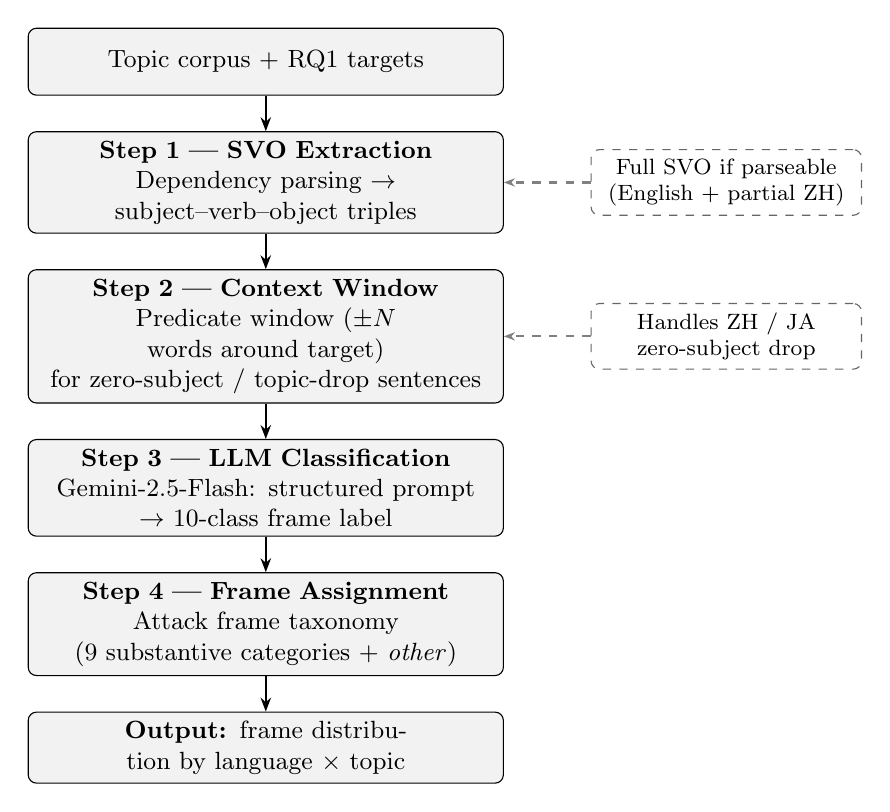
\begin{tikzpicture}[
  node distance=0.45cm and 1.4cm,
  box/.style={rectangle, rounded corners=3pt, draw=black, fill=gray!10,
              text width=5.8cm, align=center, minimum height=0.85cm, font=\small},
  sidebox/.style={rectangle, rounded corners=3pt, draw=black!60, fill=white,
                  text width=3.2cm, align=center, minimum height=0.75cm,
                  font=\footnotesize, dashed},
  arr/.style={-{Stealth[length=5pt]}, thick},
  sarr/.style={-{Stealth[length=4pt]}, thick, dashed, gray}
]

\node[box] (inp)  {Topic corpus + RQ1 targets};

\node[box, below=of inp]  (svo)  {\textbf{Step 1 — SVO Extraction}\\Dependency parsing $\rightarrow$ subject--verb--object triples};

\node[box, below=of svo]  (ctx)  {\textbf{Step 2 — Context Window}\\Predicate window ($\pm N$ words around target)\\for zero-subject / topic-drop sentences};

\node[box, below=of ctx]  (llm)  {\textbf{Step 3 — LLM Classification}\\Gemini-2.5-Flash: structured prompt\\$\rightarrow$ 10-class frame label};

\node[box, below=of llm]  (tax)  {\textbf{Step 4 — Frame Assignment}\\Attack frame taxonomy\\(9 substantive categories + \textit{other})};

\node[box, below=of tax]  (out)  {\textbf{Output:} frame distribution by language $\times$ topic};

% side annotations
\node[sidebox, right=1.1cm of svo] (ann1) {Full SVO if parseable\\(English + partial ZH)};
\node[sidebox, right=1.1cm of ctx] (ann2) {Handles ZH / JA\\zero-subject drop};

\draw[arr] (inp) -- (svo);
\draw[arr] (svo) -- (ctx);
\draw[arr] (ctx) -- (llm);
\draw[arr] (llm) -- (tax);
\draw[arr] (tax) -- (out);

\draw[sarr] (ann1.west) -- (svo.east);
\draw[sarr] (ann2.west) -- (ctx.east);

\end{tikzpicture}
\caption{RQ2 frame classification pipeline. The four sequential steps transform each document into a labelled predicate--argument pair: SVO extraction captures full syntactic structure; the context window fallback recovers predicates from zero-subject sentences; the LLM maps each pair to one of ten attack frames; the taxonomy then assigns the final label.}
\label{fig:rq2-pipeline}
\end{figure}

% ------------------------------------------------------------------
\section{RQ3: Moral Motivation Projection via FrameAxis}
\label{sec:rq3}
% ------------------------------------------------------------------

RQ3 asks why anti-Christian discourse takes different forms in Chinese, Japanese, and English — specifically, what underlying moral motivations drive attacks in each language community. Rather than relying on surface-level keywords or LLM classification, we use a vector projection approach grounded in Moral Foundations Theory (MFT) \citep{graham2009liberals}: the FrameAxis method \citep{Kwak_2021}, extended with Intergroup Threat Theory \citep{stephan2000integrated}.

\subsection{Moral Foundations and Axis Construction}

Moral Foundations Theory posits that moral intuitions are organized along five basic dimensions: Harm/Care, Fairness/Reciprocity, Loyalty/Betrayal, Authority/Subversion, and Sanctity/Degradation \citep{graham2009liberals}. We augment these five foundations with two additional axes derived from Intergroup Threat Theory: Realistic Threat (resource competition and political control) and Symbolic Threat (cultural invasion and identity erosion). These two additions are motivated by the specific context of anti-Christian hostility in East Asia, where Christianity is frequently framed as a foreign cultural agent rather than merely a set of moral beliefs.

For each axis, we define a positive pole (virtue / safety / cohesion) and a negative pole (vice / threat / degradation). The moral vocabulary for each pole is drawn from three authority dictionaries: MFD 2.0 \citep{frimer2025moral} for English, J-MFD \citep{matsuo2019development} for Japanese, and CMFD \citep{cheng_c-mfd_2023} for Chinese. For CMFD, which does not provide explicit virtue/vice polarity annotations, we infer polarity using a set of Chinese negation-prefix rules. A custom intergroup threat vocabulary covering all three languages was constructed manually based on pilot analysis of the corpus. The axis vector for foundation $k$ is then constructed as:
\begin{equation}
    \mathbf{a}_k = \text{Centroid}\!\left(\{\text{E5}(w)\}_{w \in D_k^+}\right) - \text{Centroid}\!\left(\{\text{E5}(w)\}_{w \in D_k^-}\right)
\end{equation}
where $D_k^+$ and $D_k^-$ are the positive and negative pole vocabulary sets for axis $k$, and $\text{E5}(w)$ denotes the multilingual E5-large embedding of word $w$. Each axis vector is $\ell_2$-normalized.

To make the semantic direction of each axis concrete, Table~\ref{tab:rq3_anchor_words} lists representative anchor words for both poles of every axis, with one illustrative example per language. These are the words whose centroids define the pole endpoints in E5 embedding space; any document is then located somewhere along the continuum between them.

\begin{table}[htbp]
\centering
\small
\caption{Representative anchor words defining each moral axis (EN / ZH / JA). The axis vector $\mathbf{a}_k$ is the centroid of the positive-pole embeddings minus the centroid of the negative-pole embeddings. Only a small illustrative sample is shown per cell; the last column gives the full vocabulary size $|D_k^+|$ / $|D_k^-|$ after deduplication across dictionaries.}
\label{tab:rq3_anchor_words}
\begin{tabularx}{\textwidth}{l X X r}
\toprule
\textbf{Axis} & \textbf{Positive pole (virtue / safety / cohesion)} & \textbf{Negative pole (vice / threat / degradation)} & \boldmath$|D_k^+| / |D_k^-|$ \\
\midrule
Harm/Care        & \textit{care}, \textit{protect} / 关爱, 保护 / 守る, 保護        & \textit{harm}, \textit{hurt} / 伤害, 虐待 / 傷つける, 虐待         & 1619 / 453 \\
Fairness         & \textit{fair}, \textit{justice} / 公平, 正义 / 公正, 平等        & \textit{cheat}, \textit{unfair} / 欺骗, 不公 / 不正, 差別          & 1065 / 371 \\
Loyalty          & \textit{loyal}, \textit{unite} / 忠诚, 团结 / 忠誠, 結束          & \textit{betray}, \textit{traitor} / 背叛, 叛国 / 裏切り, 背信      & 887 / 124 \\
Authority        & \textit{respect}, \textit{order} / 秩序, 尊重 / 秩序, 尊敬        & \textit{rebel}, \textit{subvert} / 反叛, 颠覆 / 反乱, 転覆         & 1782 / 226 \\
Sanctity         & \textit{pure}, \textit{sacred} / 纯洁, 神圣 / 清浄, 神聖          & \textit{corrupt}, \textit{disgust} / 污秽, 堕落 / 汚れ, 堕落       & 1171 / 538 \\
Realistic Threat & \textit{safe}, \textit{sovereign} / 安全, 主权 / 安全, 主権       & \textit{invasion}, \textit{infiltrate} / 入侵, 渗透 / 侵略, 支配   & 25 / 40 \\
Symbolic Threat  & \textit{culture}, \textit{tradition} / 文化, 传统 / 文化, 伝統    & \textit{brainwash}, \textit{cult} / 洗脑, 邪教 / 洗脳, カルト      & 25 / 33 \\
\bottomrule
\end{tabularx}
\end{table}

\subsection{Document Projection and Bias Score}

Each document $d$ in the corpus is encoded using the same multilingual E5-large model with a \texttt{passage:} prefix, producing a unit-normalized embedding. The moral bias of document $d$ along axis $k$ is then computed as the cosine similarity between the document vector and the axis vector:
\begin{equation}
    \text{Bias}(d, k) = \cos\!\left(\text{E5}(d),\; \mathbf{a}_k\right)
\end{equation}
Formally, a negative bias score indicates that the document's semantic content is closer to the negative (vice/threat) pole, while a positive score indicates alignment with the positive (virtue/safety/cohesion) pole. Crucially, however, the sign of the bias score reflects \emph{which moral vocabulary the document activates}, not the speaker's evaluative stance toward any particular target. A hostile document can score positive on Sanctity if it invokes purity or tradition language — for example, ``we must protect our sacred traditions from this cult'' — because the document's embedding is dominated by virtue-pole terms even though the overall communicative intent is to attack.

Anti-religious discourse therefore admits two distinct moral-argumentative grammars, both of which are hostile and both of which the bias framework can capture:
\begin{itemize}
    \item \textbf{Direct-condemnation grammar:} the speaker loads vice vocabulary onto the target (\textit{harmful}, \textit{unjust}, \textit{corrupt}, \textit{degenerate}). The document's semantic centre of mass shifts toward the negative pole, yielding a \emph{negative} bias on the relevant MFT axis. The target is explicitly cast as the violator of that moral value.
    \item \textbf{Identity-defense grammar:} the speaker invokes ingroup virtue vocabulary to justify the attack (\textit{our tradition}, \textit{our order}, \textit{our purity}) and simultaneously casts the target as a threat to those virtues (\textit{foreign cult}, \textit{brainwashing sect}, \textit{cultural invasion}). The document shifts \emph{toward} the positive pole of the classical MFT axes and \emph{away} from the positive pole of the threat axes, yielding a characteristic \emph{positive-MFT + negative-threat} configuration.
\end{itemize}
Neither configuration is inherently more hateful than the other; they are two rhetorical strategies for morally grounding an attack. A central motivation for projecting onto seven complementary axes — rather than collapsing to a single hostility dimension — is precisely that this structural difference between direct-condemnation and identity-defense framing becomes visible in the data, and can be compared across languages and topics. This formulation follows the original FrameAxis paper \citep{Kwak_2021} and is conceptually related to the word embedding association tests used in bias research \citep{Caliskan_2017}.

\subsection{Statistical Analysis and Interpretation}

Bias scores are computed for all documents and aggregated at the language $\times$ topic level. Cross-linguistic differences in moral motivation profiles are assessed using one-way ANOVA for each axis, with language as the grouping variable. We report $F$-statistics, $p$-values, and effect sizes ($\eta^2$) to distinguish statistically significant from incidental differences.

Because the five MFD foundations are empirically highly correlated within our corpus (pairwise correlations $\approx 0.8$), we treat them as a single ``moral-foundation bundle'' for interpretation purposes — its sign indicates whether the dominant grammar in a given slice of the data is direct-condemnation (negative bundle) or identity-defense (positive bundle) — and focus on the Realistic Threat and Symbolic Threat axes as the primary additional dimensions that differentiate language communities from one another. Within each language, we additionally compute per-topic $z$-scores to identify which topics are most strongly associated with each moral motivation, independently of the language-level baseline.

\begin{figure}[h]
\centering
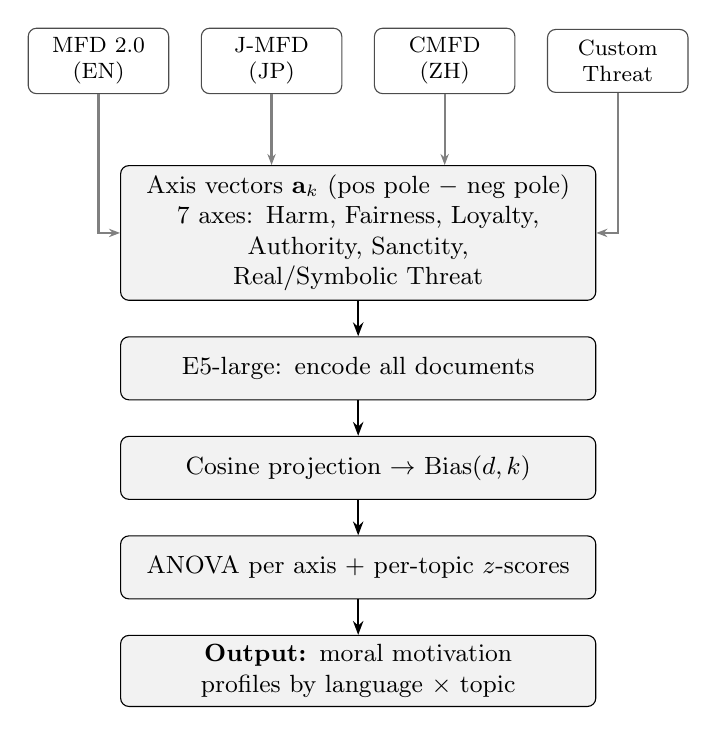
\begin{tikzpicture}[
  node distance=0.45cm and 0.5cm,
  box/.style={rectangle, rounded corners=3pt, draw=black, fill=gray!10,
              text width=5.8cm, align=center, minimum height=0.8cm, font=\small},
  dictbox/.style={rectangle, rounded corners=3pt, draw=black!70, fill=white,
                  text width=1.55cm, align=center, minimum height=0.8cm,
                  font=\footnotesize},
  arr/.style={-{Stealth[length=5pt]}, thick},
  darr/.style={-{Stealth[length=4pt]}, thick, gray}
]

% --- Dictionary Row (Layer 1) ---
\node[dictbox] (mfd)  {MFD 2.0\\(EN)};
\node[dictbox, right=0.4cm of mfd]  (jmfd) {J-MFD\\(JP)};
\node[dictbox, right=0.4cm of jmfd] (cmfd) {CMFD\\(ZH)};
\node[dictbox, right=0.4cm of cmfd] (cust) {Custom\\Threat};

\node[box, below=0.9cm of jmfd, xshift=1.1cm] (axis)
      {Axis vectors $\mathbf{a}_k$ (pos pole $-$ neg pole)\\ 7 axes: Harm, Fairness, Loyalty,\\ Authority, Sanctity, Real/Symbolic Threat};

% --- Pipeline Nodes (Layer 3-6) ---
\node[box, below=of axis] (enc)  {E5-large: encode all documents};
\node[box, below=of enc]  (proj) {Cosine projection $\rightarrow$ Bias$(d,k)$};
\node[box, below=of proj] (stat) {ANOVA per axis + per-topic $z$-scores};
\node[box, below=of stat] (out)  {\textbf{Output:} moral motivation profiles by language $\times$ topic};

\draw[darr] (mfd.south)  |- (axis.west);
\draw[darr] (cust.south) |- (axis.east);

\draw[darr] (jmfd.south) -- (jmfd.south |- axis.north);
\draw[darr] (cmfd.south) -- (cmfd.south |- axis.north);

\draw[arr] (axis) -- (enc);
\draw[arr] (enc)  -- (proj);
\draw[arr] (proj) -- (stat);
\draw[arr] (stat) -- (out);

\end{tikzpicture}
\caption{RQ3 moral motivation pipeline. Multilingual moral dictionaries define seven semantic axes; documents are projected onto these axes via cosine similarity; statistical analysis reveals cross-lingual differences in moral framing.}
\label{fig:rq3-pipeline}
\end{figure}

\subfilebibliography
\end{document}
